%!TEX root = ../Thesis.tex
\chapter{Introduction}

%\begin{itemize}
%    \item \textup{Upright shape}
%    \item \textit{Italic shape}
%    \item \textsl{Slanted shape}
%    \item \textsc{Small Caps shape}
%    \item \textmd{Medium series}
%    \item \textbf{Bold sereies}
%    \item \textrm{Roman family}
%    \item \textsf{Sans serif family}
%    \item \texttt{Typewriter family}
%\end{itemize}

%\begin{algorithm}
%\caption{Modified mini-batch $K$-means} \label{modifiedminibatch}
%\begin{algorithmic}[1]
%\State Given: $K$, mini-batch size $B$, iterations $T$, dataset $X$, correlation~matrix~$\mathrm{P}$.
%\State Initialize $C = \{\mathbf{c}^{(1)}, \mathbf{c}^{(2)}, \ldots, \mathbf{c}^{(K)}\}$ with random $\mathbf{x}$'es picked from $X$.
%\State $A \gets B \cdot T$ sorted random indexes to $X$, denoted $a_1, a_2, \ldots, a_{B\cdot T}$.
%\State $X' \gets \{\mathbf{x}^{(a_1)}, \mathbf{x}^{(a_2)}, \ldots, \mathbf{x}^{(a_{B\cdot T})}\}$ \Comment{Cache all points}
%\State $\textbf{size} \gets 0$
%\For {$i = 1$ to $T$}
%    \State $M \gets B$ examples picked randomly from $X'$
%    
%    \For{$\mathbf{x} \in M$} \Comment{\textit{Assignment step}}
%        \State $\textbf{d}[\textbf{x}] \gets f(C,\mathbf{x}, \mathrm{P})$ \Comment{Cache closest center}
%    \EndFor
%    
%    \For {$\mathbf{x} \in M$} \Comment{\textit{Update step}}
%        \State $\textbf{c} \gets \textbf{d[x]}$ \Comment{Get cached center for current \textbf{x}}
%        \State $\textbf{size}[\textbf{c}] \gets \textbf{size}[\textbf{c}] + 1$ \Comment{Update cluster size}
%        \State $\eta \gets \frac{1}{\textbf{size}[\textbf{c}]}$       \Comment{Get learning rate}
%        \State $\textbf{c} \gets (1 - \eta)\textbf{c}+\eta\textbf{x}$ \Comment{Take gradient step}
%    \EndFor
%\EndFor
%\State \Return {$C$, \textbf{size}}
%\end{algorithmic}
%\end{algorithm}

Fusce id suscipit sem. Aliquam venenatis nibh nec nisl luctus vel consectetur neque dapibus. Nulla feugiat egestas turpis, ac viverra eros cursus sit amet. Cras tincidunt felis vel tellus ultrices condimentum. Quisque vehicula, arcu vitae interdum dignissim, purus tortor cursus libero, sit amet accumsan quam magna in neque. Phasellus luctus leo odio. Aliquam ultricies, arcu quis tempor rhoncus, tellus nisl tempus justo, condimentum tempor erat odio ac purus. Integer quis ipsum felis. Aliquam volutpat, leo ac consequat egestas, lectus lacus adipiscing quam, id iaculis dolor quam in erat. Phasellus tempor interdum arcu quis vestibulum. Pellentesque sit amet augue purus. 
\begin{figure}[htbp]
    \centering
        \missingfigure[figwidth=6cm]{This is some text that is with the todo and in the figure}
    \caption{This is the caption I wrote}
    \label{fig:label}
\end{figure}
Curabitur condimentum suscipit arcu, sit amet convallis urna pellentesque ac. Quisque fringilla tincidunt risus nec accumsan. Curabitur vel sagittis ante. Integer eget placerat leo. Class aptent taciti sociosqu ad litora torquent per conubia nostra, per inceptos himenaeos. Vestibulum quis risus in nulla fermentum pellentesque dictum et erat. Nulla vel pretium nunc. Integer tortor lorem, suscipit sit amet ultricies non, porta at metus. Sed pharetra, ante facilisis interdum porta, mi dolor fringilla quam, ac porttitor urna dolor quis massa. Proin viverra semper tincidunt. Vivamus pulvinar pharetra condimentum. Pellentesque rutrum mollis tellus ac scelerisque.

%------------------------------------------------------------------------------------
\section{Sollicitudin vestibulum}
\label{sec:ch1_crap}
%------------------------------------------------------------------------------------
Mauris luctus sollicitudin vestibulum. Class aptent taciti sociosqu ad litora torquent per conubia nostra, per inceptos himenaeos. Duis eu nisl nec turpis porttitor bibendum eget sed orci. Aliquam consequat lorem a dui viverra porta facilisis augue rutrum. Cras luctus tellus in lectus egestas eu consequat magna cursus. Aenean aliquam neque a nibh elementum ornare. Integer eleifend imperdiet commodo. Morbi auctor, dui vel laoreet congue, purus est accumsan augue, sit amet feugiat neque nisl vel lorem. Curabitur ante sem, lacinia id adipiscing quis, viverra tristique nulla. Pellentesque ullamcorper pellentesque metus varius facilisis. Cras ac dui id odio tempor scelerisque. Curabitur a egestas risus. Pellentesque quis velit in sapien accumsan auctor. Phasellus aliquam, sapien eget lobortis volutpat, libero metus porttitor nisl, sed hendrerit urna dolor nec mi.

Praesent et pellentesque arcu. Phasellus venenatis mi eu lorem convallis et iaculis ante aliquet. Aenean rhoncus placerat metus, vel convallis leo suscipit eu. Integer dapibus venenatis commodo. Cras laoreet faucibus sem nec luctus. Class aptent taciti sociosqu ad litora torquent per conubia nostra, per inceptos himenaeos. Cras consectetur lacinia dolor at gravida. Phasellus ipsum arcu, vulputate fermentum ultricies eget, tempor eu odio. Aenean accumsan vestibulum risus a mattis.

\begin{adjustwidth*}{0cm}{-0.4cm}
	\begin{lstlisting}[language=Python,caption=Fibonacci2,label=Fibonacci2]
	# This is a comment
	import easy
	str = "I am a string"
	str2 = "Now i have an awsome string with ´ '' `` which are not TeX'ed"
	str3 = "What about awsome unicode characters? Like “, π, ”, Ω, ç. \" This"
	def fib(n):
	    if n == 0:
	        return 0
	    elif n == 1:
	        return 1
	    else:
	        return fib(n-1) + fib(n-2)
	str4 = "Yes it is possible with 80 charactes. Which this string proves. Wiiii."
	str5 = "It adjusts according to the spine"
	\end{lstlisting}
\end{adjustwidth*}
%------------------------------------------------------------------------------------
\section{Doppler wind lidar basics}
\label{sec:ch1_lid_basics}
%------------------------------------------------------------------------------------
Doppler Wind Lidars (DWL)... they're great (see \ref{fig:NothingElseMatters}).  
%---
\begin{figure}[h!]%[htbp]
	\centering
%	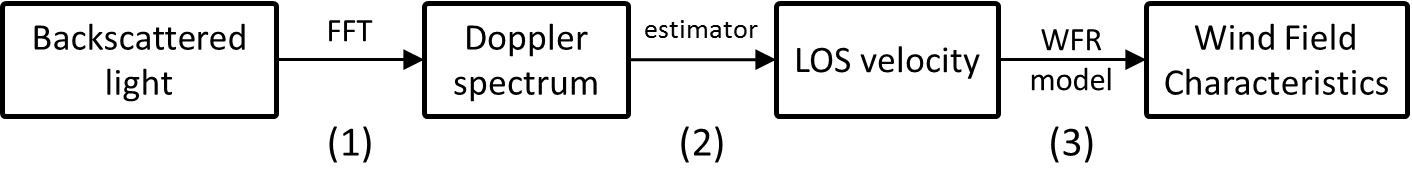
\includegraphics[height=0.08\textheight]{Lidar_MeasurementsPrinciples_V1.png}
	\missingfigure[figwidth=6cm]{BLABLABLABLABLA}
	\vspace*{-4mm}
	\caption{Another caption.}
	\label{fig:NothingElseMatters}	
	\setlength{\belowcaptionskip}{-20pt}
\end{figure}
%---
BLABLABLA. 
\\\\
More blabla.
%---
\subsection{Subsection title}
\label{subsec:ch1_subsectitle}    
%---
\textbf{\color{red}BLABLA}
%---
\subsubsection{Sub-subsection title}
\label{subsubsec:blabla1}    
%---
\textbf{\color{red}BLABLA}
%---
\subsection{Else}
\label{subsec:ch1_else}    
%---
\textbf{\color{red}BLABLA}